
Since the top quark production cross-section is substantially higher than the
diboson production cross-section, top backgrounds generally pose a significant 
challenge for dilepton plus \met analyses. To reduce the top background, 
we use a combination of two top tagging methods implemented and commissioned in the $\hww$ 
analysis~\cite{HWW2011AN}, both relying on the fact that top quarks 
decay to $Wb$ with almost certainty.

The first method vetoes events containing soft muons from the $b$-quark decays 
The requirements used to select soft muons are:
%%%%%%%%%%%%
\begin{itemize}
    \item $\pt > 3$ GeV;
    \item Reconstructed as a TrackerMuon
    \item Meets $\mathrm{TMLastStationAngTight}$ muon id requirements
    \item The number of valid inner tracker hits $>10$
    \item The transverse impact parameter with respect to the Primary Vertex, $|d_{0}| < 0.2$~cm,
    \item The longitudinal impact parameter with respect to the Primary Vertex, $|d_{z}| < 0.2$~cm,
    \item Non-isolated $({\rm{Iso}_{Total}}/{\pt}~>~0.1)$ if $\pt>20\GeV$.
\end{itemize}
%%%%%%%%%%%%

The second method uses standard $b$-jet tagging. 
The jets are reconstructed using calorimeter and tracker information using a particle flow 
algorithm~\cite{jetpas}. The anti-${\rm k_T}$ clustering algorithm~\cite{antikt} 
with ${\rm R=0.5}$ is used. We apply the standard jet energy 
corrections~\cite{jes} to the reconstructed jets, where the L1 Fast Jets 
corrections are included. The latter corrections are rather important since 
they help in flattening the reconstruction efficiency as a function of the 
number of overlapping events.
In this method, events containing jets with $E_T>30\:\GeV$ tagged with
 the $\mathrm{TrkCountingHighEff}$~\cite{btag} algorithm with
a discriminator value of greater than 2.0 are vetoed. 
	

%The algorithm is applied to jets with the same definition as Section \ref{sec:sel_jets},
%with the exception that the $E_T$ requirement is removed. 
%Thus, events in the zero-jet bin can still contain tagged jets.

%As a comparison of performance , the $\WW$ signal efficiency versus the $\ttbar$ efficiency in 
%events with no jets according to the definition in Section \ref{sec:sel_jets} for different 
%standard b-tagging algorithms  is shown in Figure~\ref{fig:eff_btag_tt_ww}. 
%For a top rejection efficiency above $40\%$,
%the $\mathrm{TrkCountingHighEff}$ tagger performs better than the others.
%Our current cut value has a $\WW$ signal efficiency of about $98.1\%$ and
%a $\ttbar$ efficiency of about $39\%$.

%%%%%%%%%%%%
%\begin{figure}[!htbp]
%\begin{center}
%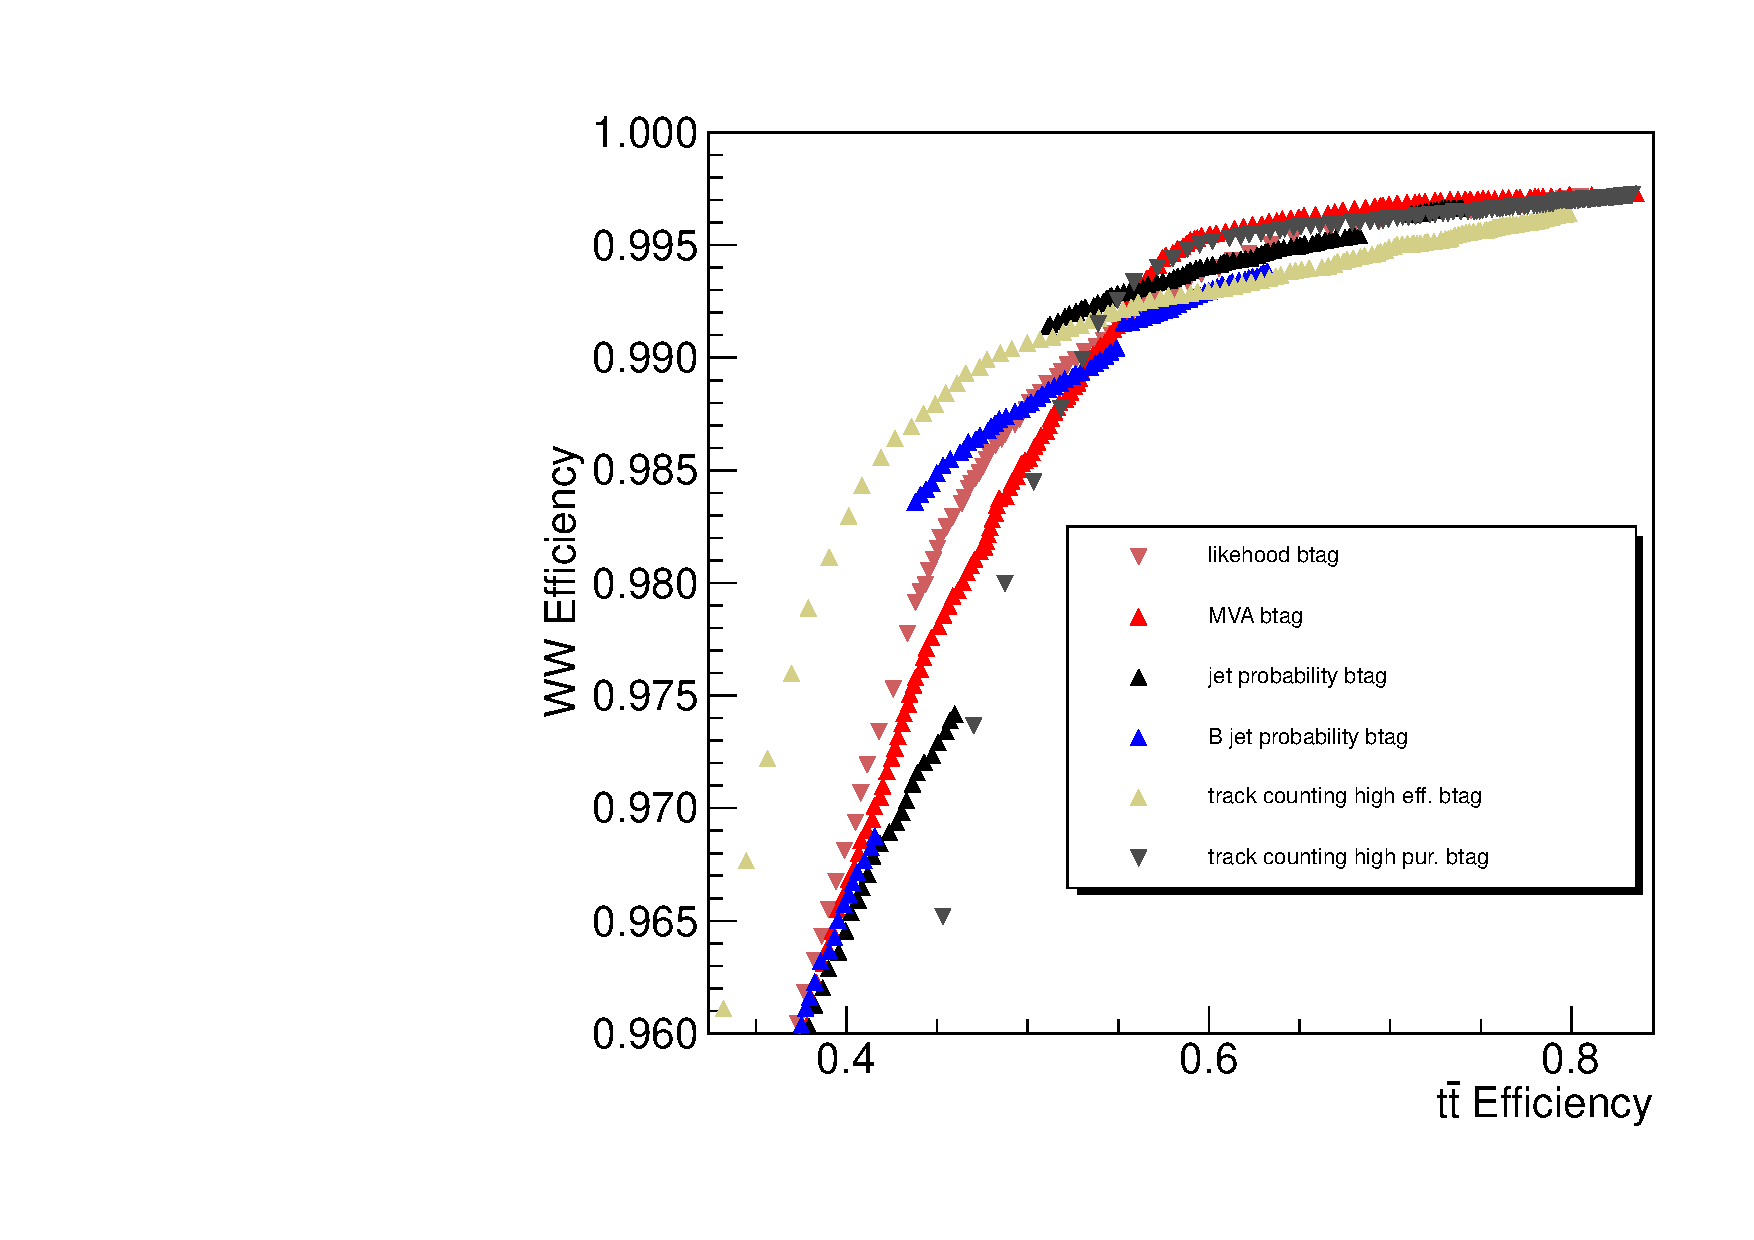
\includegraphics[width=0.60\textwidth]{figures/eff_btag_tt_ww.pdf}
%\caption{$\WW$ signal efficiency versus $\ttbar$ efficiency in events with no
%reconstructed jets for different standard b-tagging algorithms.}
%\label{fig:eff_btag_tt_ww}
%\end{center}
%\end{figure}
%%%%%%%%%%%%

%By using the expected tagging efficiency for the two methods,
%it is possible to estimate the residual top background after the vetoes
%have been applied. 
%This is described in detail in Section \ref{sec:bkg_top}.
